\chapter{Implementation}
\section{Overall approach to implementation}
This chapter discusses the implementation of the music social network app 'Dynamic'. It is split into  multiple stories which have previously been listed in Chapter 1. Not all of the stories are discussed here as some stories were very similar to others.

\section{Toolset}
It was very important to use an appropriate toolset for this project. Using an appropriate toolset would not only save time but would also aid in the creation of code.

Git is one tool which was used throughout the creation of the project. Git is a very useful tool as it not only allows for just backups but also for version control \cite{git}. The main difference being version control means that all different revisions of the project could be viewed; this is extremely useful as it means that if the app code was to break, then the code could be restored to a working version. There are many different applications of git, consequently there are multiple providers of git services including Gitlab and Github \cite{github} \cite{gitlab}. For this project Github was used. As shown in Figure 3.1 a private git repository was set up which is what what used for version control and back ups.
\begin{center} 
\begin{figure}[H]
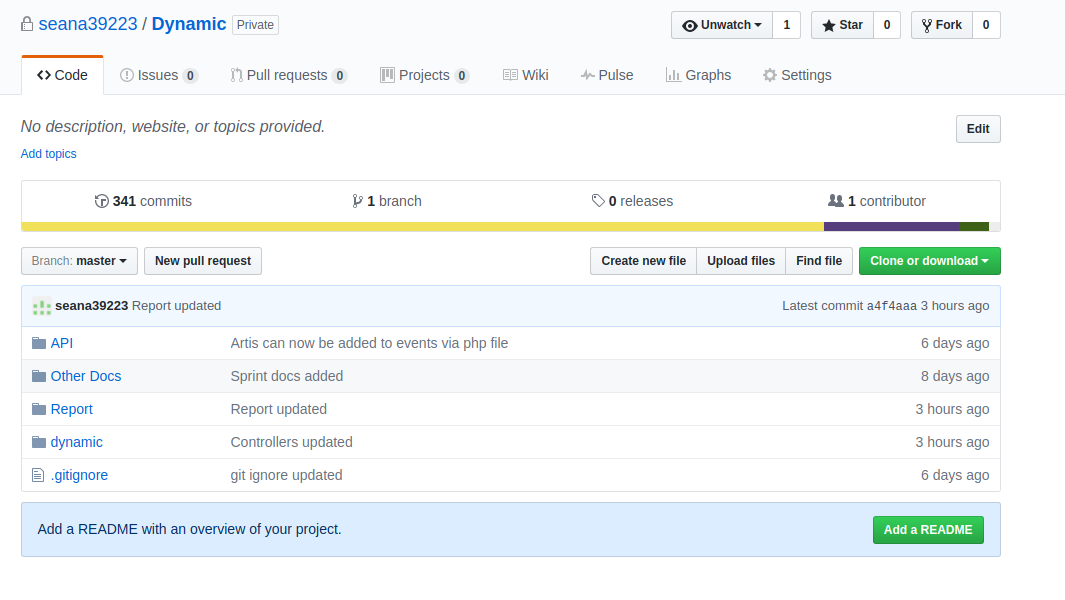
\includegraphics[scale=0.3]{images/git}
\caption{Git repository}
\end{figure}
\end{center}

Sublime is the text editor which was chosen for the project. Sublime was chosen as it has a large range of plugins, which are able to check the syntax of code along with tabulation etc. This is better than using a basic text editor such as vim as it makes producing the code easier.

\section{The Registration system}
\subsection{Back End}
Work began on the registration system by creating the appropriate tables in the back end database. These tables were user\_types, users, genres and user\_genres. The user\_types table contained the three different types of account which a user could have: Music Lover, Artist and Venue Owner and an id associated with each of these. The user type was implemented as a separate table to the users table itself for extensibility purposes as if additional user types needed to be added then they could simply be added to this table. The users table just contained all of the users' details including name, display name, email, password (discussed in more depth during the security section) and a url link to their profile picture. The genres table was simply a table which contained different genres of music and an appropriate id for each genre. As genres to users is a many to many relationship a users\_genres table was created which stores a user\_id and a genre\_id.

After the tables had been created, the php files (hosted at \url{seananderson.co.uk/api}) were created. These php files essentially formed the RESTful API which would allow for the front end to connect to the database for this system. The first file which was created was register.php. This file takes variables which the user passes in (through POST data) and adds them to the database via my sqli commands which are run from within the php. This file automatically gives the user a generic picture url of a gingerbread man \cite{ginger}. Some validation was done in the php file to check that things such as emails given are valid email addresses, however most of the validation was done on the front end as this would allow for error messages to reach the user in a quick manner. 

As at this stage in time there was no front end, consequently it was not possible to test that sending POST data from the app would work. So, a piece of software called postman (which is a Google Chrome extension) was used. This software allows for POST data to be pushed to a website or API as illustrated in Figure 3.2. As well as relying on the PHP file telling me 'A new user was added successfully' which is the message what is printed when the sql commands all run correctly, the database was also checked to ensure that the new user had been added correctly as shown in Figure 3.3.

\begin{center} 
\begin{figure}[H]
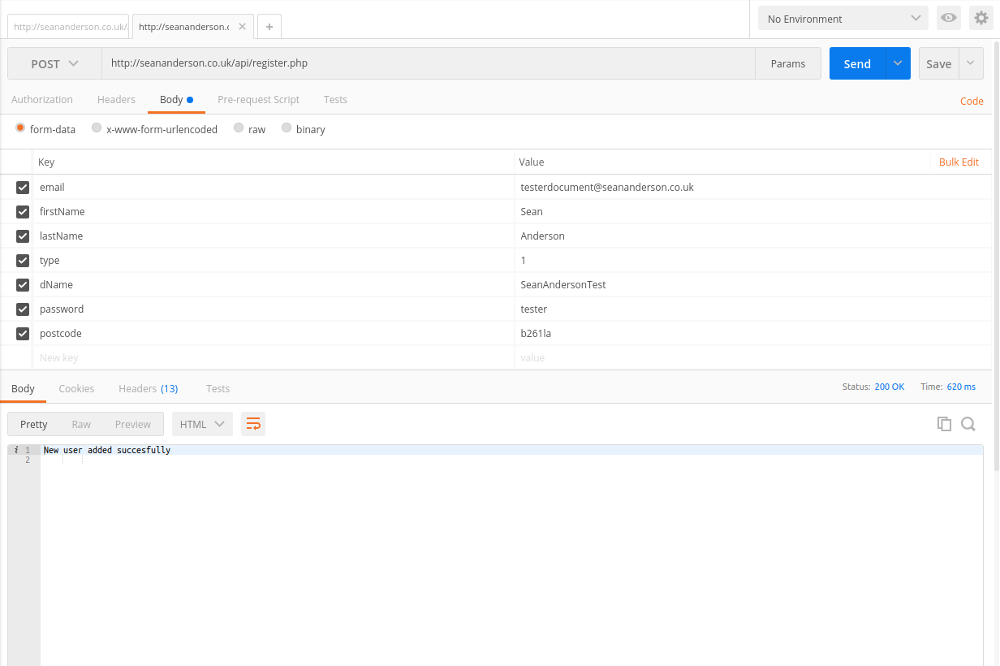
\includegraphics[scale=0.45]{images/postman}
\caption{Postman testing register.php}
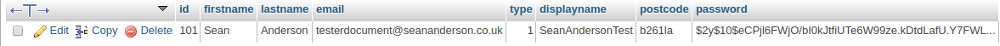
\includegraphics[scale=0.45]{images/db1}
\caption{User added to the database}
\end{figure}
\end{center}

\subsubsection{Security within the registration system}
It is important that users are not allowed to enter dangerous characters into the database, as a result of this all strings which are inputted by the user are escaped using the mysqli\_escape function which is a default php function which ensures that any characters which could potentially do damage to the database are escaped and therefore not ran in the mysqli statements.

As the registration and login system used a password it was important to ensure that if somebody was to get access to the database that they wouldn't get access to the password. There are multiple different methods of encryption which could have been used for this. PHP has its own built in function called password\_hash which takes in two parameters the password itself as a string and the encryption type. For this project password\_default which is a predefined php hashing method was used. Password default was used as it was a simplistic and relatively secure way of turning a password into a hash. The password\_verify function in PHP is used to check that a plain text password matches the hashed password.
 
\subsection{Front end}
After the back end for the registration of the app was created, development then started on the front end. The default ionic menu bar template was used as this would allow for a menu bar to appear on multiple pages (like in the design) easily.

The views for both the login and registration system were created using html (as are all views in ionic) and the controllers for these views were created in AngularJS and were simply js files. Both the register and login view files contained a form which gathered appropriate information from the user and then passed that information onto the controllers when submitted. The controllers then passed that information onto the API's by using \$http.post which is an AngularJS method used for calling post API's. Figure 3.4 shows how the AngularJS controller passes the appropriate data to the API. The full code for the registration system is shown in Appendix 3.
\begin{center}
\begin{figure}[H]
\begin{verbatim}
$http.post(api, data).then(function(res){
  apiReturns = JSON.stringify(res);
  if (apiReturns.includes('New user added succesfully')>=0) {
    localStorage.setItem('email', $scope.register.email);
    localStorage.setItem('dName', $scope.register.dName);
    if ($scope.registerGenre!=undefined) {
      $scope.registerGenre();
    }
    $state.go('app.profile');
    popUp('Welcome', 'Welcome to Dynamic please fill in 
    your profile page and then follow some users');
  }
})
\end{verbatim}
\caption{AngularJS code for posting to register account}
\end{figure}
\end{center}

In passing the information from the controller to the API I encountered a problem. AngularJS sends post data in a different way to most other languages. As a result of this the following lines of code had to be added to the PHP files as shown in Figure 3.5. (This code was taken from \url{http://corpus.hubwiz.com/2/angularjs/15485354.html})
\begin{center} 
\begin{figure}[H]
\begin{verbatim}

if ($_SERVER['REQUEST_METHOD'] == 'POST' && empty($_POST)) {
    $_POST = json_decode(file_get_contents('php://input'), true);
}
\end{verbatim}
\caption{Code to make API work properly}
\end{figure}
\end{center}

Figure 3.6 shows what the front end for the login and registration screens look like on the front end on the system (from the perspective of a One Plus Two device.)
\begin{center}
\begin{figure}[H]
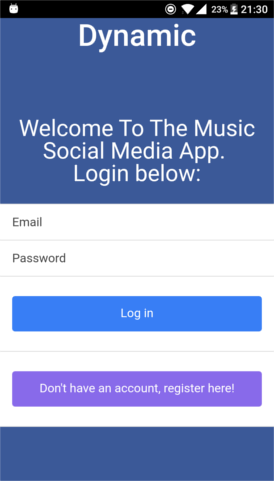
\includegraphics[scale=0.5]{images/sc1}
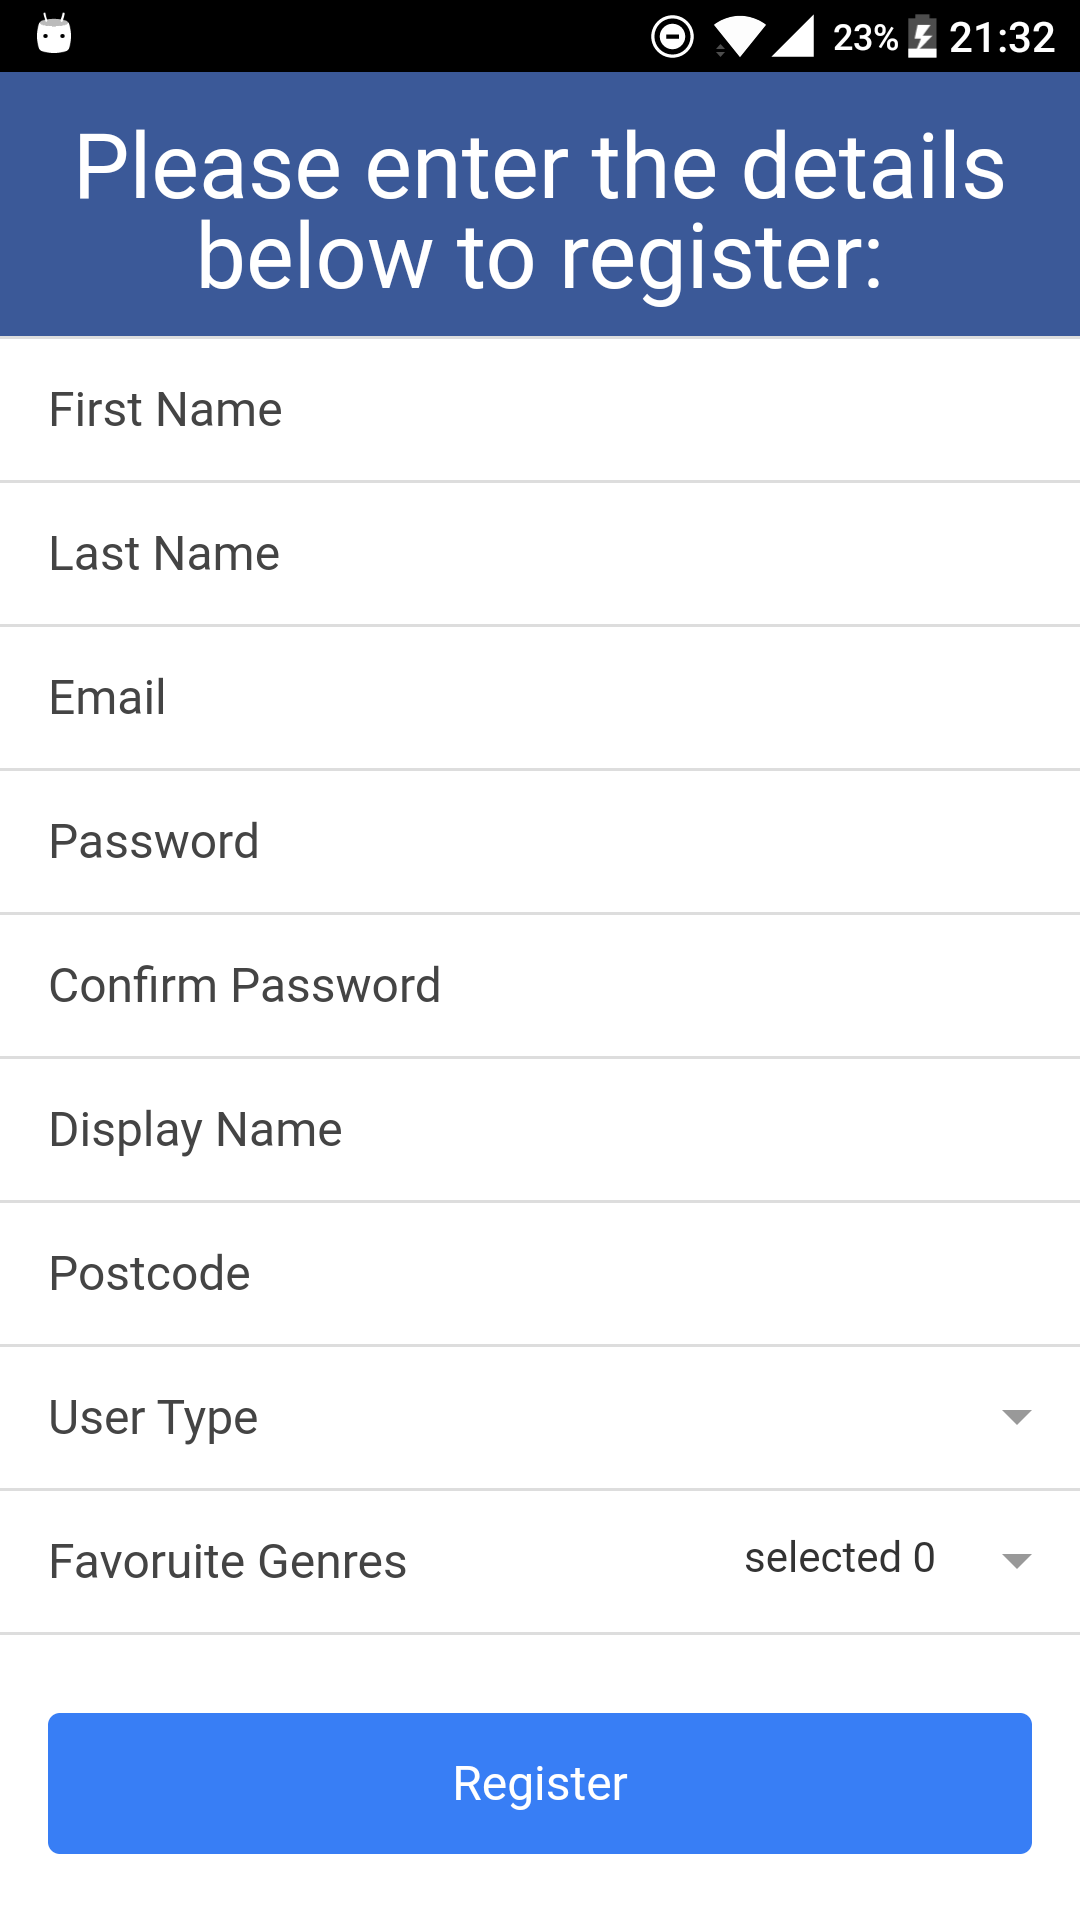
\includegraphics[scale=0.5]{images/sc2}
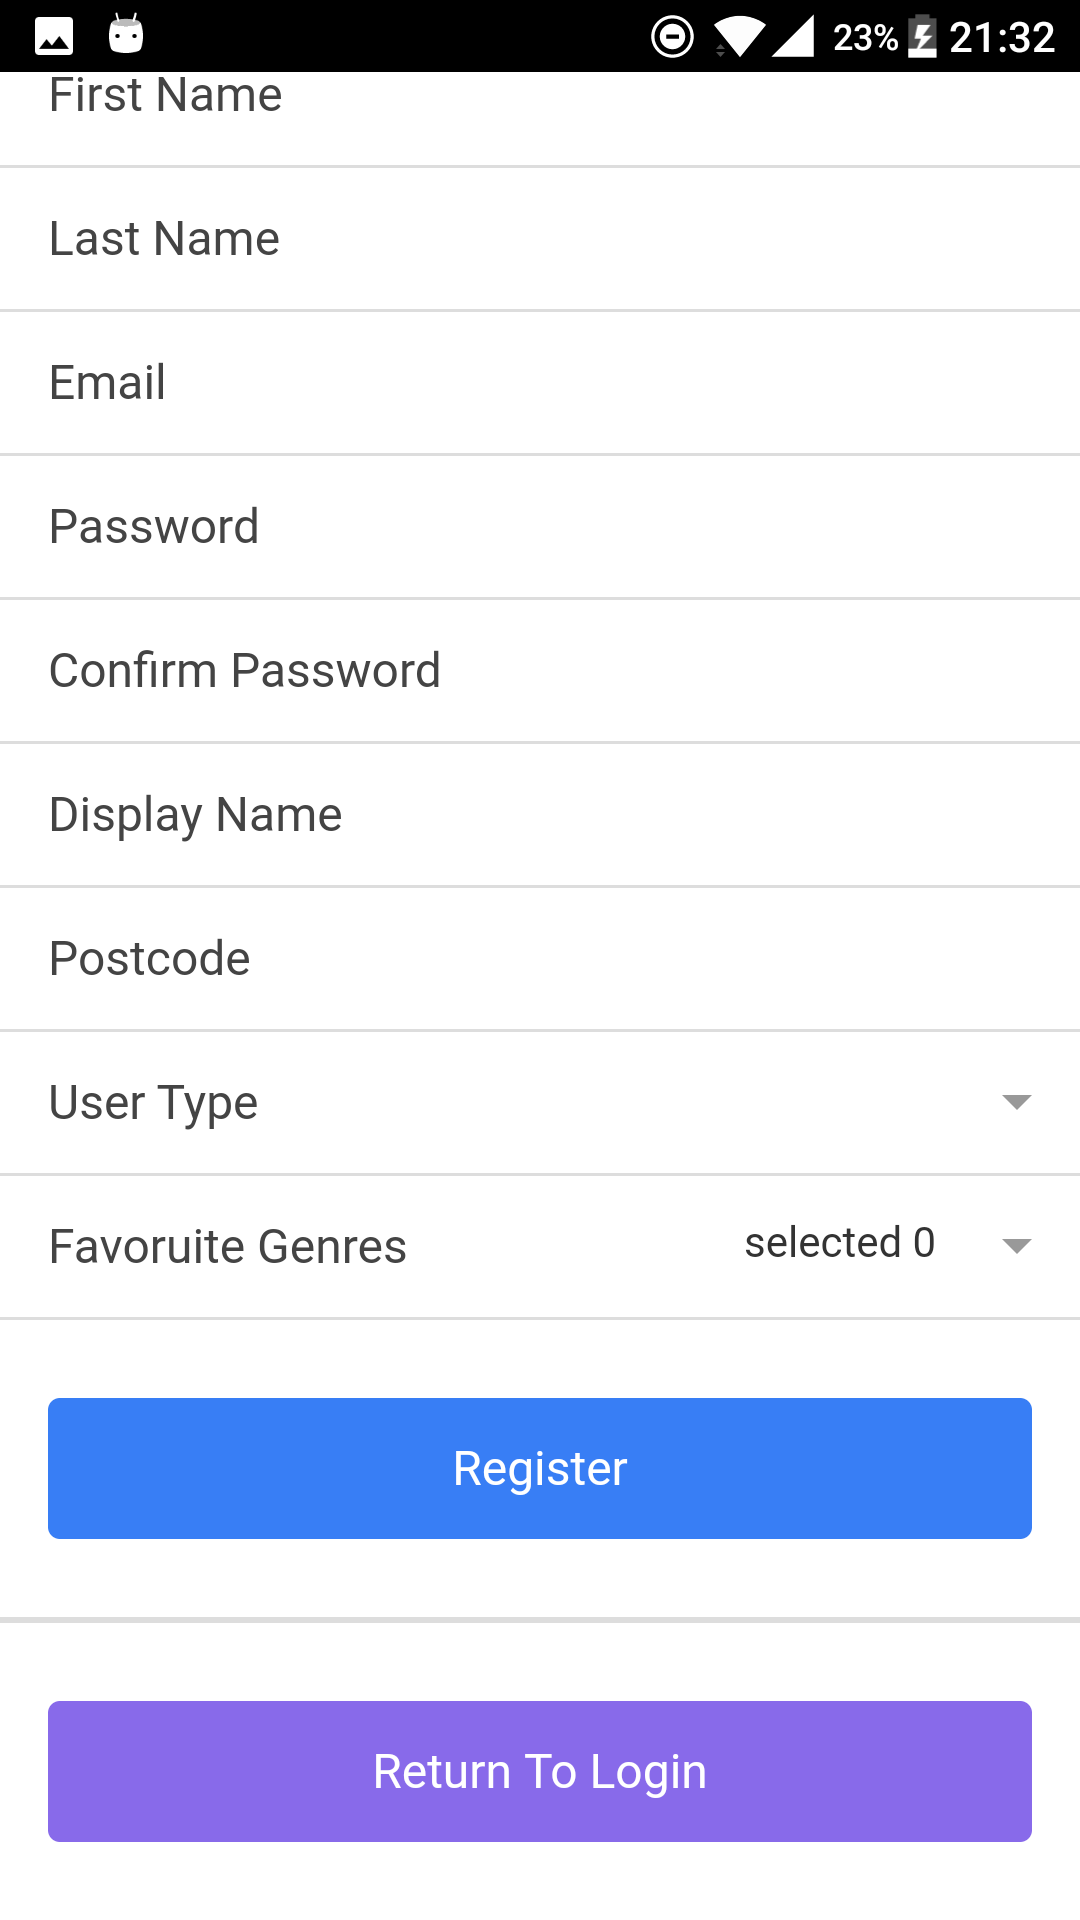
\includegraphics[scale=0.5]{images/sc3}
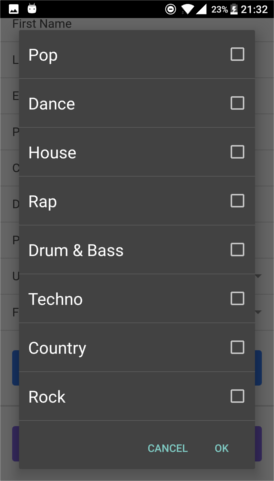
\includegraphics[scale=0.5]{images/sc4}
\caption{Screenshots of registration system.}
\end{figure}
\end{center}

\subsection{Validation}
Having successfully got the front end interacting with the back end it was important to ensure that all of the data being sent over was valid. I decided first of all to validate the data on the front end. This ensured that the user had filled in all of the appropriate boxes and a regular expression was used to ensure that the email address they entered was valid.

It was then necessary to create some more API files as each user had to have a unique email and display name, files called checkemail.php and displayname.php were created. These files run SQL queries to ensure that the email address and display name which the user entered are unique.

Figure 3.7 displays an example of what happens when a user tries to register an account with an email address which has already been used and when a password is not long enough.
\begin{center}
\begin{figure}[H]
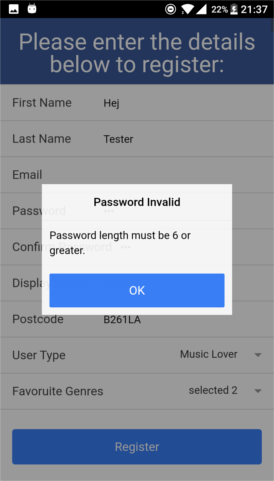
\includegraphics[scale=0.5]{images/sc5}
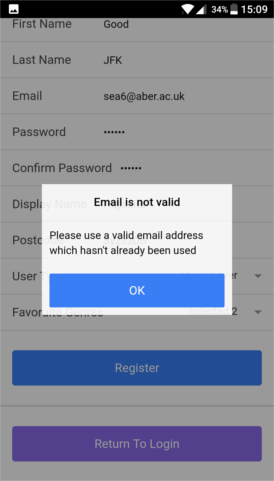
\includegraphics[scale=0.5]{images/sc6}
\caption{Validation Screenshots}
\end{figure}
\end{center}

\section{Posting to a feed}
There were multiple ways in which a user posting to a feed could be carried out. It was decided that a users posts would be stored in the database and would be retrieved from the database at appropriate times. As the relationship between a user and a post is a many to many relationship, a new table was created in the database called feed. 

An API file called feed.php was created, this file takes in two post variables a users email and a users post (the string the user would like to add to their feed.) This file then uses the users email and runs a sql command to get the users id. This id is then placed into the feed table along with the users post variable.

The front end of the system worked in a way which was very similar to the registration system. The view of the front end was simply a text input field and a button (as shown in Figure 3.8) which when clicked would call an action in the controller.

This controller would then pass the appropriate variables to the API, using \$http.post in the same way as the registration system. Finally a message would display to the user to let them know they had posted, this is shown in Figure 3.8.
\begin{center}
\begin{figure}[H]

\includegraphics[scale=0.5]{images/sc10}
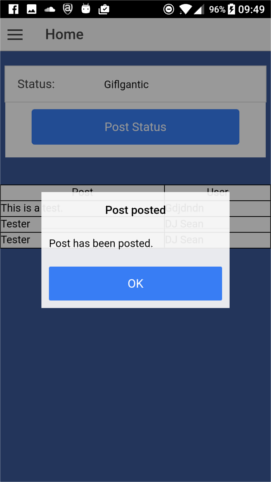
\includegraphics[scale=0.5]{images/sc11}
\caption{Validation Screenshots}
\end{figure}
\end{center}

\section{Creation of Events}
An important component of the mobile application was that users with the type venue owner could create events. Creating events is split into two different parts, actually adding the venue where events will take place to the app and then the actual creation of an event.

\subsection{Adding a Venue}
The purpose of adding a venue to the app is so that a venue owner can quickly create multiple events at the same venue and they don't have to enter the venue's details every time. The system for adding a venue was designed in a way that should be simple for the venue owner to add a new venue. They simply had to navigate to the 'Add a Venue' page and enter the appropriate details as shown in Figure 3.9. 

The system worked in the same way as the registration system in how it passes the data to the back end.
\begin{center}
\begin{figure}[H]
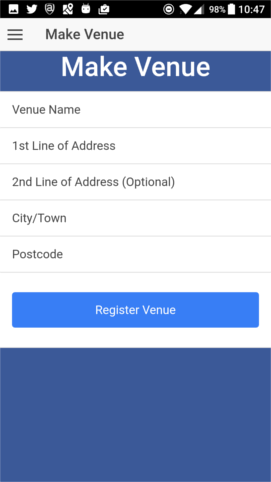
\includegraphics[scale=0.5]{images/sc12}
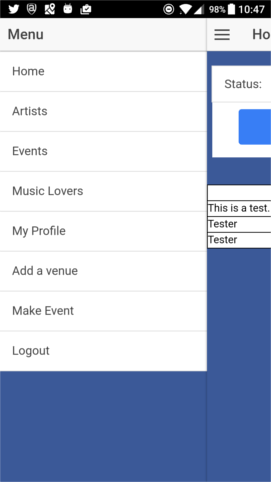
\includegraphics[scale=0.5]{images/sc13}
\caption{Front End for adding a venue}
\end{figure}
\end{center}

\subsection{Adding an Event}
Adding an event requires the user to already have a venue associated with them, consequently a message is displayed telling the user to add a venue if they don't already have one as shown in Figure 3.10.
\begin{center}
\begin{figure}[H]

\includegraphics[scale=0.5]{images/sc14}
\caption{Message which displays if the user has no venue.}
\end{figure}
\end{center}

Then once the user has created a venue they can create an event. The user simply fills in the appropriate details to create an event. The three drop down options on the page event venue, closest genre of event and artists performing are populated through API's. In terms of the event venue an API is called which gives all of the venues associated with the user logged in. The closest genre of the event is simply all of the genres which are in the database and the artists performing at event is made up of all artists who have an account on the app as shown in Figure 3.11. Once the details the user has entered are validated, in that all of the information they have provided is valid (correct) the event is then added to the app and both music lovers and venue owners can add events to their favourites. 
\begin{center}
\begin{figure}[H]
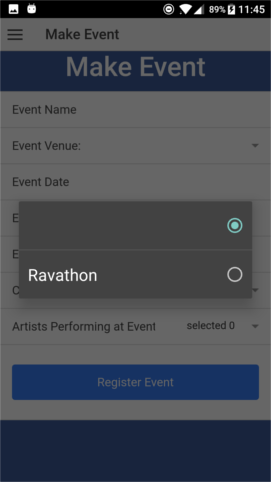
\includegraphics[scale=0.5]{images/sc16}
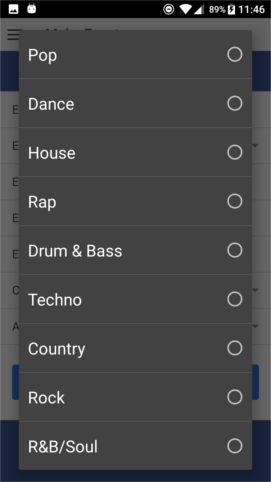
\includegraphics[scale=0.5]{images/sc17}
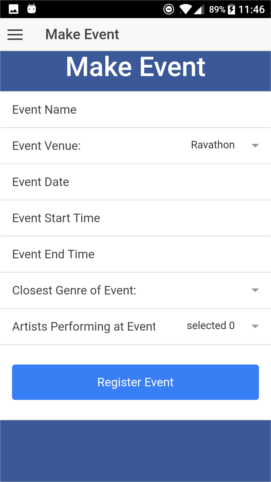
\includegraphics[scale=0.5]{images/sc18}
\caption{Creating an event}
\end{figure}
\end{center}

\section{Users profile}
Having created the registration and login system the next story which was tackled was allowing the user to add a bio and to upload a picture. This picture would act as the users profile picture. Having previously completed the registration system allowing the user to add a bio was rather straightforward. It was just simply a matter of creating a front end which passes a variable to a php file (called update bio.php), the php files then takes the post variable and turns it into a php variable. Finally as shown in figure X the php file runs a sql command which updates the users table to have the correct information for the bio.

\begin{figure}[H]
\begin{verbatim}
$sql = "UPDATE users SET bio = '$bio' WHERE displayname = '$dName' ";
\end{verbatim}
\caption{Snippet of updatebio.php code which shows SQL command.}
\end{figure}

\subsection{Camera and FileTransfer plugins}
The task of allowing a user to upload a profile picture can be broken down into two seperate tasks. The task of actually allowing the user to take the photo or pick a photo from their devices library, and the task of transferring that photo to the back end. 

Installing the cordova camera plugin \cite{cc} was necessary to allow the user to take a photo or select a photo from their devices library. The actual installation of the plugin was simple, following the documentation for the plugin was straightforward and the app was programmed so that if the user clicked a button saying upload a picture or choose a picture from my gallery then the Cordova Camera plugin was called with the correct options configured.

Figure 3.12. highlights the two different buttons and what happens when they are clicked.
\begin{center}
\begin{figure}[H]

\includegraphics[scale=0.5]{images/cs}
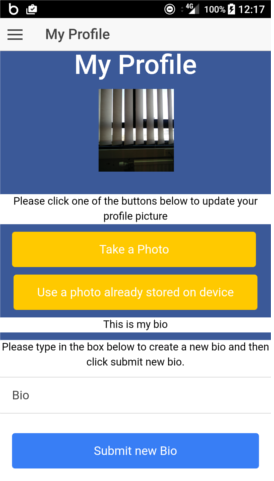
\includegraphics[scale=0.5]{images/sc7}
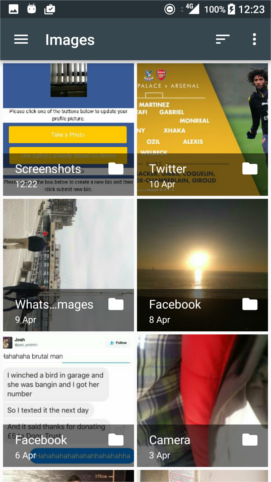
\includegraphics[scale=0.5]{images/sc9}
\caption{Screen shot of camera functionality.}
\end{figure}
\end{center}

After the user confirms (by pressing the tick) that they want to use the photo as their profile picture the photo is then uploaded to the server. The first step in getting the photo to upload was to create a API file, this file was entitled imageupload.php and is hosted at \url{seananderson.co.uk/api/imageupload.php}. This file contains some fairly trivial code which just gets the data of the image which has been uploaded and places it in an appropriate folder (\url{seananderson.co.uk/api/uploads}). After creating the php file the next step was to pass the photo from the device to the server. This was done by using the Cordova File Transfer plugin \cite{ft}. This plugin simply takes a file (which in this case was the image) and uploads the file to the specified URL.

After implementing the camera plugin one clear disadvantage of hybrid apps became apparent. The time taken for the device to take a picture and then process that picture was noticeably longer than it takes when using a native app such as Facebook. This is discussed in more depth during the testing section of this report. 

\subsection{Caching issue}
At this stage of the development of the app it became apparent that there was an issue with caching. The issue was when the picture was loaded onto the users profile page after the user uploaded a new picture, the picture would not be updated and would display the users old display picture even though the new image had successfully been uploaded. 

A variety of different ways were used to try and tackle this issue. Ionic allows for the apps cache to be cleared using \$ionicHistory.clearCache(); however this unfortunately didn't resolve this issue. As clearing the apps cache wasn't getting rid of the issue it was clear that the problem lay within the browser (which is how the app is ran.)

It turned out that the Chrome browser was caching the results of the API which displayed the picture, as the same API was being called on the page refresh, which was ran once the photo was uploaded. Despite not being the most elegant solution a random number was added to the end of the pictures url as shown in Figure 3.13.
\begin{center}
\begin{figure}[H]
\begin{verbatim}
$http.post(api, data, { cache: false }).then(function(res){
  //Below line is a hack, justified in report.
  var image = (res['data']['picture']) + '?random=' + Math.random();
  var photoDiv = angular.element(document.querySelector('#profile-photo'));
  photoDiv.html('<div id ="profile-photo"><img  height="60 px" 
  width="60 px" src="' + image + '"</img></div>');
})
\end{verbatim}
\caption{AngularJS Photo Code.}
\end{figure}
\end{center}

This meant that the browser would load the new image uploaded into the app as it would have a different url from the old image. The caching issue is clearly a negative to hybrid app development, if the app was developed in a native manner then it would allow for the developer to have full control over the cache and therefore this issue would not have arose had the app been developed in a native manner. 

\subsubsection{Problem with Different Devices}
The camera plugin worked fine on a One Plus Two mobile phone, however when the camera was tested using a Samsung Galaxy A there was a problem, the orientation of the image was wrong. The Samsung Tablet would take the photo fine but when it actually came to uploading it, it would rotate the image. 

One of the options when using the camera plugin is photo orientation as shown in Figure 3.14. 
\begin{center}
\begin{figure}[H]
\begin{verbatim}
var options = {
  quality:80,
  targetWidth:500,
  targetHeight:750,
  sourceType : Camera.PictureSourceType.CAMERA,
  encodingType: Camera.EncodingType.PNG,
  correctOrientation: true
};
\end{verbatim}
\caption{Camera Plugin Options.}
\end{figure}
\end{center}
Unfortunately enabling that to be true still didn't solve the problem. Despite there not being any official sources suggesting why the correct orientation doesn't always work the feeling within the Ionic Community is that Samsung devices actually ignore the correctOrientation option \cite{ioniccom1}. This is clearly another disadvantage to hybrid apps as native apps would give the developer more control \cite{androidcamera}.
\section{Styling and porting over to iOS}
As ionic uses HTML for its views, the styling is done in CSS, SASS can be used as an alternative to CSS if the developer wants. The majority of the app was styled whilst working on each story however it was important to spend some time to ensure that the styling of the app was consistent across multiple devices and platforms.

iOS mobile applications can only be released and launched through using xCode which is only available on Macs. Clearly this requires some effort however it requires significantly less effort than if the apps were developed in a native manner. If the apps were developed in a native manner then the code would have to be completely rewritten for launch on iOS devices where as when using a hybrid technology it is simply a matter of installing any plugins on the Mac which were installed when developing the Android version and potentially some slight tweaks to the styling as Android and iOS browsers interpret CSS slightly differently. 

This did actually bring up some issues with hybrid app development. Whilst a key feature of hybrid app development is the ability to deploy an app to multiple different code bases; iOS and Android interpret CSS differently. Therefore time had to be spent tweaking the CSS of the iOS version. (Add this if possible Figure X shows a particular part of the app running on iOS and Android however it is clearly inconsistent.)

\begin{figure} [H]
\caption{iOS not the same as Android image goes here}
\end{figure}


\section{Recommendation System}
When creating the recommendation system it was considered that information about the user to recommend events can be obtained explicitly and implicitly \cite{ML}. It was important to consider that if the app was released commercially then the ethics of obtaining data implicitly would need to be considered and the user would need to understand exactly how their data would be used.

The recommendation system was made for events and in terms of explicit data available, two pieces of information were relevant these were the users favourite genre's of music and the users postcode. This is because each event has a genre associated with it and a postcode so comparing this information allows for the establishment of how similar in terms of music the user likes is to the event and the distance between the user and the event. When using the explicit data to recommend events the system would be using content based filtering \cite{san}.

There was only one relevant type of implicit data available about users which would help in creating a recommendation system, this is the users current favourite events. If the user has already chosen to favourite a event then it is possible to compare the events they currently have favourite with other events and make recommendations based of how similar the events are. When using implicit data to recommend events the system would be using collaborative filtering algorithms \cite{collab}.

\subsection{Content Based Filtering}
The recommendation system runs when the user decided to sort events by recommended events. The first thing which happens when the user does this is that the app makes a call to the back end which checks if the user has any events in their favourites. If they do have events in their favourites then the system uses collaborative filtering algorithms to recommend events if not it uses the following method to recommend events using content based filtering.
\begin{enumerate}
  \item Looks up genres of music associated with the user.
  \item Looks to see if any of those genres of music are being played at events and adds appropriate events to an array.
  \item Sorts the array in terms of distance between the users home and event.
  \item Displays the recommended events on the app itself.
\end{enumerate}
Figure X shows how steps 1 and 2 work via php code (the full code can be seen in Appendix 4 under recommendedevents.php).
\begin{figure}
\begin{verbatim}
$sql = "SELECT genre_id from user_genres WHERE user_id = '$userId'";
$genres = $connection->query($sql) or trigger_error($mysqli->error."[$sql]");
    foreach ($genres as $genre) {
        $genreIdSql = $genre['genre_id'];
        $sql = "SELECT * from events WHERE genre_id = '$genreIdSql'";
        $events = $connection->query($sql) or trigger_error($mysqli->error."[$sql]");
        while($event = mysqli_fetch_assoc($events)) {
            $eventsArray[] = $event;
        }
    }
}
\end{verbatim}
\caption{Code which shows how steps 1 and 2 work for Content Based Filtering}
\end{figure}
Figure X shows how the events display on the front end of the app once they have been sorted.
\begin{figure}
\caption{Insert figure showing sorted events here.}
\end{figure}

\subsection{Collaborative filtering}
When the user does have some favourite events, collaborative filtering is performed to give the user recommended events. As with the content based filtering this process was split into multiple steps.
\begin{enumerate} 
  \item All of the users favourite events are added to an array.
  \item An empty array is created called recommended events.
  \item A calculation is then performed to calculate the similarity between the events which the user hasn't got as favourites and the events they have got as favourites.
  \item Events which the user doesn't have as favourites are added to the recommended events array in order of how similar they are to the events which the user has already placed as favourites.
\end{enumerate}
The calculation for similarity between events consists of two main things; the genre of the event and the location of the event. This calculation is essentially an implementation of the K Nearest Neighbour(k-NN) machine learning algorithm \cite{knn} \cite{knn2}. K-nn is a useful machine learning algorithm which can be used to classify data, it was implemented in such a way to this project so that an event which is near to an event which a user is attending would be a recommended event to a user.

\section{Debugging and other features of hybrid app development}
One massive advantage of the ionic framework is that the developer can actually launch the app in a Google Chrome browser by running the 'ionic serve' command from a terminal. This is a very useful feature as it also allows for code to be edited and the page will simply refresh as shown in Figure 3.15. This is a clear positive of hybrid app development as it means that the code can be 'live edited' so the developer can see the changes they are making and because the user doesn't necessarily have to use emulators which can be resource heavy.
\begin{center}
\begin{figure}[H]
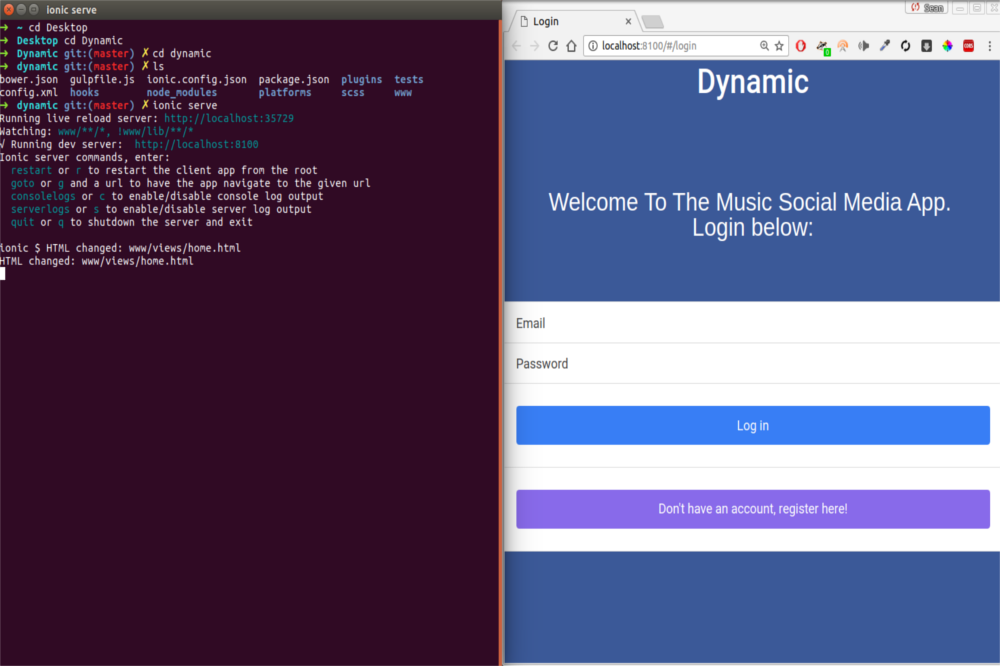
\includegraphics[scale=0.45]{images/chrome}
\caption{ionic serve command running}
\end{figure}
\end{center}

Debugging the app is also rather straightforward as Google Chrome's developer tools can be opened up whilst running ionic serve as shown in Figure 3.16 this allows for various commands to be typed to test a variety of things and also for console logs to be displayed which clearly aids the developer in checking variables.
\begin{center}
\begin{figure}[H]
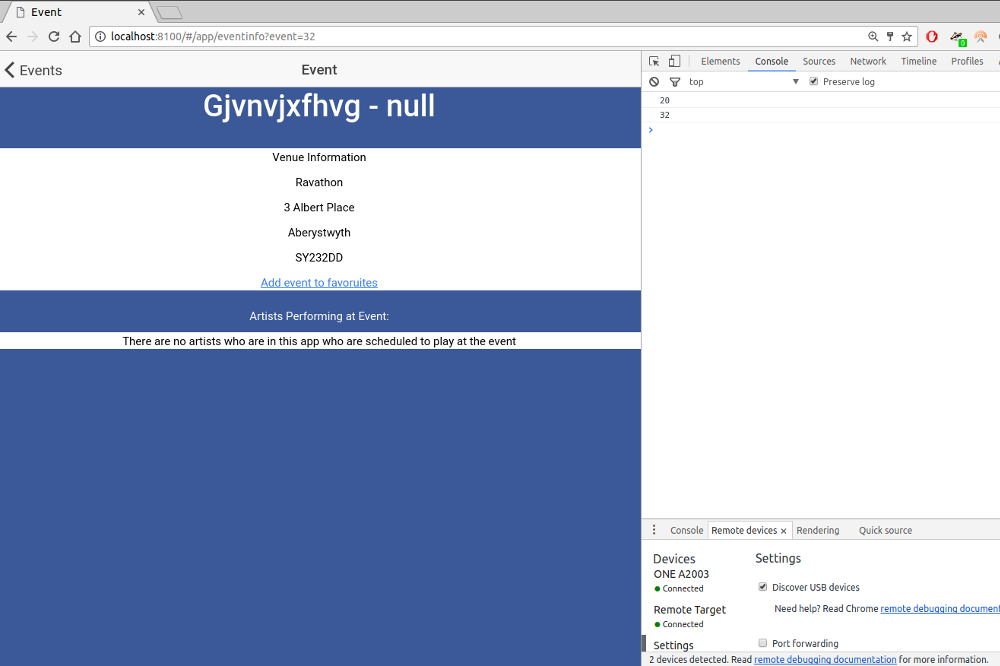
\includegraphics[scale=0.45]{images/chrome2}
\caption{Chrome developer tools}
\end{figure}
\end{center}

\section{PHP files}
The back end of the app had over 30 PHP files, this had clearly taken a lot of time to develop. There is a lot of overlap in the files and a lot of them are very similar they just perform slightly different functions. When the system was initially thought of it wasn't expected that there would be so many PHP files and that is why all of the files were wrote manually, rather than using a framework. 

This is where using an agile approach for the project had a negative impact, as if a plan driven approach had been used then it would have been realised much earlier on in the project the sheer amount of PHP files which would have to be created and so an appropriate framework would have been selected.

\section{Technical challenges}
There was multiple technical challenges which were faced when developing the app. The first of which was actually learning AngularJS, this was simply a case of trying different things until they worked and looking at multiple different sources online.

The caching issue was a rather interesting technical challenge, despite it not taking a long time to resolve it clearly highlighted an issue with hybrid mobile apps. The photo orientation with the multiple different devices was also an issue as it meant that more lines of php had to be added to the API to ensure that the photo was uploaded in right orientation, therefore a developer would have to spend more time working on the photo upload using hybrid technologies than if they were to use the native app development.

\section{Implementation vs design and plan}
The advantage of using an agile methodology as opposed to a plan driven methodology was that if the initial plan was not the best option the project could easily be changed. Generally the initial plan and design of the system did end up being part of the implementation however in certain circumstances the plan was not adhered to. These include 
\begin{itemize}
  \item Slight changes to how venue and event creation work, so that a venue has to be created before an event.
  \item When the project was thought of initially the amount of PHP files without using a framework was vastly underestimated.
\end{itemize}
As a whole whilst the implementation didn't always stick to the design and plan it did stick to the initially planed stories and requirements.
\section{Conclusion of implementation}
Overall the implementation of the creation of the app went well. The actual development of the app meant that many advantages and disadvantages to hybrid app development could be established. The main advantages which were discovered were: quicker to port over than a native app would be, easy to use tools for debugging, language was relatively straightforward to pick up for a developer with some web experience and the app does seem to be relatively fast. Some of the disadvantages which were discovered include: not having full control over platform native features such as a cameras orientation, having very little control over memory usage of a device and a few caching issues.

